\documentclass[a4paper,twoside,11pt]{article}
\usepackage{a4wide,graphicx,fancyhdr,amsmath,amssymb, enumerate, caption, subcaption, wrapfig}

%----------------------- Macros and Definitions --------------------------

\setlength\headheight{20pt}
\addtolength\topmargin{-10pt}
\addtolength\footskip{20pt}

\newcommand{\HRule}{\rule{\linewidth}{0.5mm}} % Defines a new command for the horizontal lines,
\newcommand{\N}{\mathbb{N}}
\newcommand{\ch}{\mathcal{CH}}

\fancypagestyle{plain}
\fancyhf{}
\fancyhead[LO,RE]{\sffamily\bfseries\large Technische Universiteit Eindhoven}
\fancyhead[RO,LE]{\sffamily\bfseries\large 2IV35 Visualization}
\fancyfoot[LO,RE]{\sffamily\bfseries\large Department of Mathematics and Computer Science}
\fancyfoot[RO,LE]{\sffamily\bfseries\thepage}
\renewcommand{\headrulewidth}{0pt}
\renewcommand{\footrulewidth}{0pt}


\pagestyle{fancy}
\fancyhf{}
\fancyhead[RO,LE]{\sffamily\bfseries\large Technische Universiteit Eindhoven}
\fancyhead[LO,RE]{\sffamily\bfseries\large 2IV35 Visualization}
\fancyfoot[LO,RE]{\sffamily\bfseries\large Department of Mathematics and Computer Science}
\fancyfoot[RO,LE]{\sffamily\bfseries\thepage}
\renewcommand{\headrulewidth}{1pt}
\renewcommand{\footrulewidth}{0pt}


\begin{document}
\begin{titlepage}

\center % Center everything on the page

\textsc{\Huge \textbf{Technische Universiteit Eindhoven}}\\[1.5cm] % Name of your university/college
\textsc{\LARGE \textbf{Visualization}}\\[0.5cm] % Major heading such as course name
\textsc{\large 2IV35}\\[0.5cm] % Minor heading such as course title

\HRule \\[0.4cm]
{ \huge \bfseries Visualization data of the Netherlands}\\[0.4cm] % Title of your document
\HRule \\[1.5cm]

\begin{minipage}{0.4\textwidth}
\begin{flushleft} \large
\emph{\textbf{Author:}}\\
Sander Kools \\
0848523 \\
s.w.a.kools@student.tue.nl % Your name
\end{flushleft}
\end{minipage}
~
\begin{minipage}{0.4\textwidth}
\begin{flushright} \large
\emph{\textbf{Author:}}\\
Luuk Hulten\\
0720248 \\
l.a.j.v.hulten@student.tue.nl
\end{flushright}
\end{minipage}\\[4cm]

{\large \today}\\[3cm] % Date, change the \today to a set date if you want to be precise

\vfill % Fill the rest of the page with whitespace

\end{titlepage}

\newpage
\tableofcontents
\newpage

\section*{Information Visualization}
In this report we will describe how we implemented a web application for visualizing a large data set for the course 2IV35. This data set contains information about the population living in the Netherlands.  \newline
There is a wide variation of data, for instance the percentage of age range or car usage. The data is very large and it is hard to understand the data when viewed in the tabular view as it was provided, therefore we have come up with a better interface to make viewing and understanding the provided data easier. \newline
In section 1, we will first give a description of the format of the data set. \newline
In section 2, we will explain our design considerations for the interface. \newline
In section 3, we will present our actual implementation, with screenshots and motivation. \newline
In section 4, we will consider the trends found in the visualization. \newline
Finally in section 5, we will give a short conclusion about how we choose to visualize the data. \newline
\newline
\newline
\newline
\newline
\newline
\begin{figure}[h]
  \begin{center}
    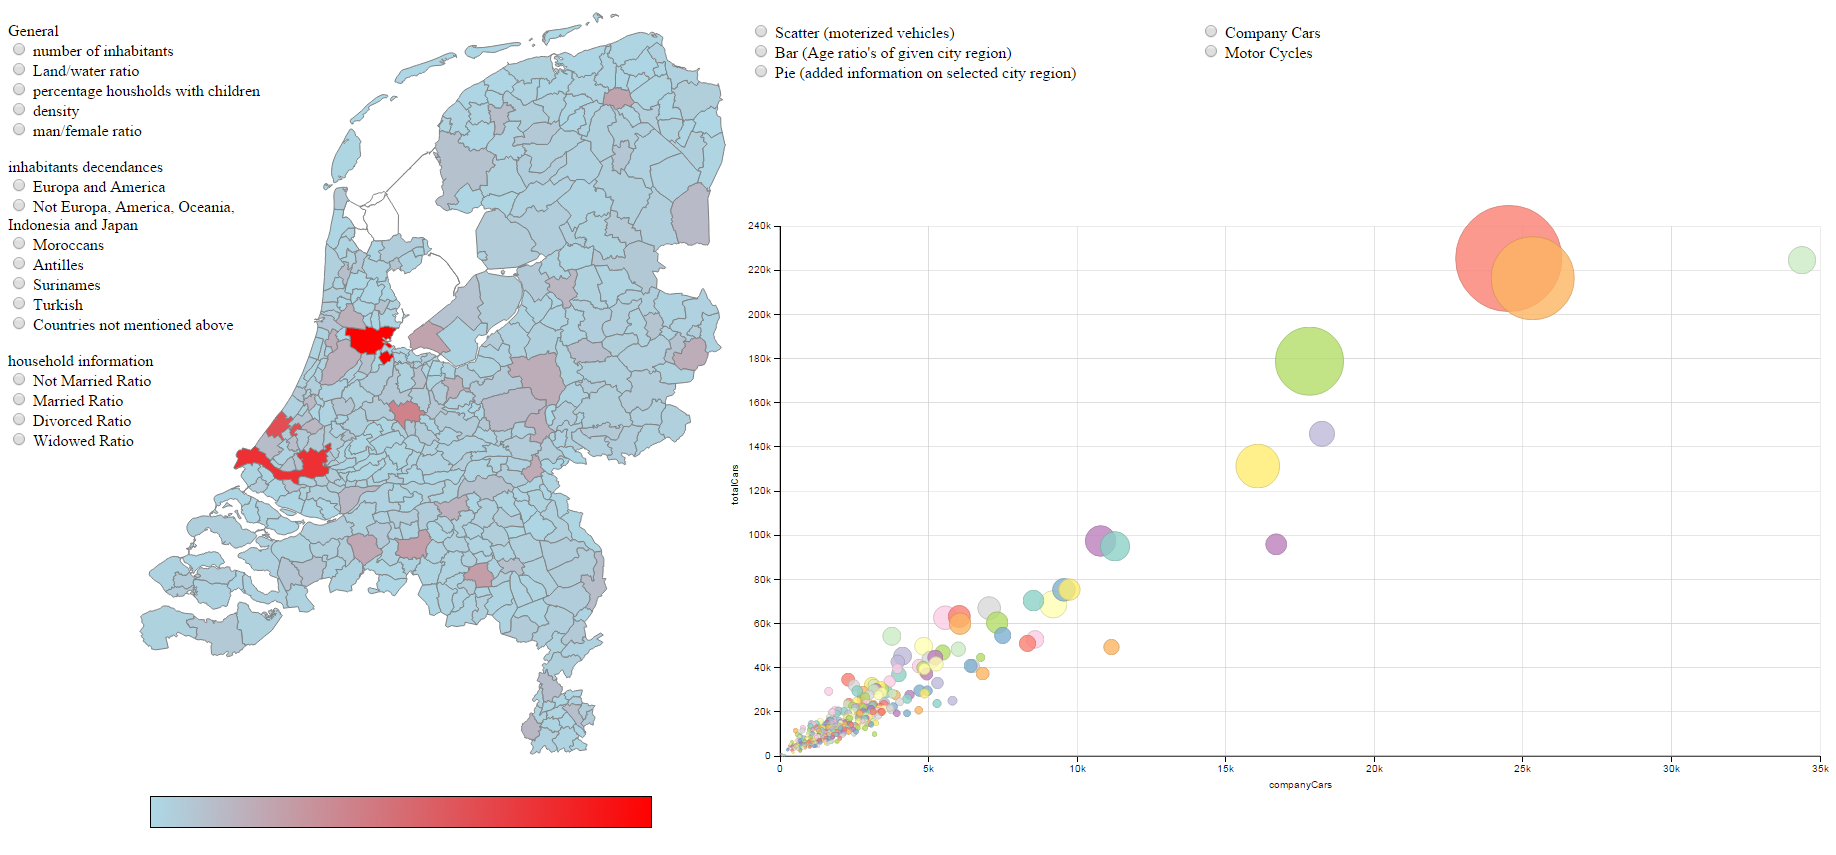
\includegraphics[width=1\textwidth]{FullScreen2}
  \end{center}
  \caption{Overview of our application, showing two modes next to each other. Here we see the map of the Netherlands with population given in heatmap next to the scatter plot of total number of cars against company cars.}
\end{figure}

\section{Description of the Dataset}
We have been given a dataset with information about the population living in the Netherlands. The data is provided in a .txt file with 417 rows and 60 columns, every column is separated by a tab. Every row represents a city region of the Netherlands. This region is also describe inside a json file listing the coordinates of the region so that it can be drawn, all the regions combined represents the Netherlands.
\subsection{High-level description}
Our data set is called "cities-data.txt" and it describes various data about city regions in the Netherlands. The data is very detailed, for instance there is data given on the percentage of people between 0-14, 15-24, 25-44, 45-65 and 65 and older. but also a more detailed percentage is given of people between 0-4, 5-9 all the way to 95 and older. \newline
The other data that is included is from the number of people and the density, surface area of land and water, descendance of the inhabitants, married and not married people, divorced people, widowed people, children in the household and number of cars, company cars or motorcycles. All the data is given for every city region. A detailed list of the data available can be seen in the subsection Description of the format found below. \newline
\subsection{Description of the format}
The dataset originates from http://www.opencbs.nl, and it consists of shape information of Dutch municipalities in GEOJson format (cities-geometry.json), and a
tab-separated file containing many statistics of these municipalities (cities-data.txt). \newline
The following statistics are provided: \newline
\begin{center}
    \begin{tabular}{ | p{4.9cm} | p{10cm} |}
    \hline
    \textbf{Column name} & \textbf{Description} \\ \hline
        GM\_NAAM [string] & The official name of the municipality \\ \hline
        WATER [] & Has no relevance here \\ \hline
        OAD [number] & Average number of addresses per square kilometer \\ \hline
        STED [number] & Describes the urban character using the following classification: \newline
                        1 very strongly urban ≥ 2500 addresses per km2 \newline
                        2 strongly urban 1500 − 2500 addresses per km2 \newline
                        3 moderately urban 1000 − 1500 addresses per km2 \newline
                        4 slightly urban 500 − 1000 addresses per km2 \newline
                        5 not urban < 500 addresses per km2  \\ \hline
        AANT INW [number] & Number of inhabitants \\ \hline
        AANT MAN [number] & Number of inhabitants \\ \hline
        AANT VROUW [number] & Number of women \\ \hline
        P 00 14 JR [percentage] & Percentage of inhibations aged 0 to 15 years \\ \hline
        P 15 24 JR [percentage] & Percentage of inhibations aged 15 to 25 years \\ \hline
        P 25 44 JR [percentage] & Percentage of inhibations aged 25 to 45 years \\ \hline
        P 45 64 JR [percentage] & Percentage of inhibations aged 45 to 65 years \\ \hline
    \end{tabular}
\end{center}
\begin{center}
    \begin{tabular}{ | p{4.9cm} | p{10cm} |}
        \hline
        \textbf{Column name} & \textbf{Description} \\ \hline
        P 65 EO JR [percentage] & Percentage of inhibations aged 65 years and older \\ \hline
        P ONGEHUWD [percentage] & Percentage of unmarried people \\ \hline
        P GEHUWD [percentage] & Percentage of married people \\ \hline
        P GESCHEID [percentage] & Percentage of divorced people \\ \hline
        P VERWEDUW [percentage] & Percentage of widows and widowers \\ \hline
        BEV DICHTH [number] & Number of inhabitants per km2 \\ \hline
        AANTAL HH [number] & Number of households \\ \hline
        P EENP HH [percentage] & Percentage of single households \\ \hline
        P HH Z K [percentage] & Percentage of households without children \\ \hline
        6P HH M K [percentage] & Percentage of households with children \\ \hline
        GEM HH GR [number] & Average number of people in all households \\ \hline
        P WEST AL [percentage] & Percentage of foreigners from Europe, North-America, Oceania, Indonesia, and Japan \\ \hline
        P N W AL [percentage] & Percentage of foreigners not from Europe, North-America, Oceania, Indonesia, and Japan \\ \hline
        P MAROKKO [percentage] & Percentage of foreigners from Morocco, Ifni, Spanish Sahara, and Western Sahara \\ \hline
        P ANT ARU & Percentage of foreigners from the Dutch Antilles and Aruba \\ \hline
        P SURINAM [percentage] & Percentage of foreigners from Surinam \\ \hline
        P TURKIJE [percentage] & Percentage of foreigners from Turkey \\ \hline
        P OVER NW [percentage] & Percentage of foreigners from other countries than mentioned in the above 4 attributes \\ \hline
        AUTO TOT [number] & Number of cars \\ \hline
        AUTO HH [number] & Number of cars per household \\ \hline
        AUTO LAND [number] & Number of cars per km2 \\ \hline
        BEDR AUTO [number] & Number of company cars (minivans, trucks, etc \\ \hline
        MOTOR 2W [number] & Number of motorcycles, including scooters \\ \hline
        OPP TOT [number] & Total land and water area in hectares \\ \hline
        OPP LAND [number] & Land area in hectares \\ \hline
        OPP WATER [number] & Water area in hectares \\ \hline
        P 00 04 JR [percentage] & Percentage of inhibations aged 0 to 5 years \\ \hline
        P 05 09 JR [percentage] & Percentage of inhibations aged 5 to 10 years \\ \hline
        P 10 14 JR [percentage] & Percentage of inhibations aged 10 to 15 years \\ \hline
        P 15 19 JR [percentage] & Percentage of inhibations aged 15 to 20 years \\ \hline
        P 20 24 JR [percentage] & Percentage of inhibations aged 20 to 25 years \\ \hline
        P 25 29 JR [percentage] & Percentage of inhibations aged 25 to 30 years \\ \hline
        P 30 34 JR [percentage] & Percentage of inhibations aged 30 to 35 years \\ \hline
        P 35 39 JR [percentage] & Percentage of inhibations aged 35 to 40 years \\ \hline
        P 40 44 JR [percentage] & Percentage of inhibations aged 40 to 45 years \\ \hline
        P 45 49 JR [percentage] & Percentage of inhibations aged 45 to 50 years \\ \hline
        P 50 54 JR [percentage] & Percentage of inhibations aged 50 to 55 years \\ \hline
        P 55 59 JR [percentage] & Percentage of inhibations aged 55 to 60 years \\ \hline
    \end{tabular}
\end{center}
\begin{center}
    \begin{tabular}{ | p{4.9cm} | p{10cm} |}
        \hline
        \textbf{Column name} & \textbf{Description} \\ \hline
        P 60 65 JR [percentage] & Percentage of inhibations aged 60 to 65 years \\ \hline
        P 65 69 JR [percentage] & Percentage of inhibations aged 65 to 70 years \\ \hline
        P 70 74 JR [percentage] & Percentage of inhibations aged 70 to 75 years \\ \hline
        P 75 79 JR [percentage] & Percentage of inhibations aged 75 to 80 years \\ \hline
        P 80 84 JR [percentage] & Percentage of inhibations aged 80 to 85 years \\ \hline
        P 85 89 JR [percentage] & Percentage of inhibations aged 85 to 90 years \\ \hline
        P 90 94 JR [percentage] & Percentage of inhibations aged 90 to 95 years \\ \hline
        P 95 EO JR [percentage] & Percentage of inhibations aged 95 years and older \\ \hline
    \end{tabular}
\end{center}
The data is delivered as a .txt file with columns that are separated with a tab. There is a lot of data to choose from, although a big part of the data is about the age range percentage. Also certain parts of the data can be determined using a combination of the other data available, for instance the "STED" can be determined using the "OAD" data or "OAD" itself could be determined using the surface area and the total inhabitants.
\newpage
\section{Design}
In this section we explain the general design of the visualization.

\subsection{General design}
Since the dataset contains a large quantity of data about municipalities, a decision has to been made what to visualize. And also what visualization technique suits the selected data, so that it can be easily interpreted. More important is a valuable visualization, meaning that we can find valuable and useful information that meets the requirements.

\subsection{Graphs}
The dataset mostly consists out of percentages so displaying this distribution in a pie chart seems obvious. In a pie chart you can easily see how a group of people is divided in subgroups. However a pie chart can not contain too much data since the sections become to small and hard to distinguish. In the case of the municipalities data married, divorced, widower and singles is an good example to represent in a pie chart. Since there are not too many categories presented in percentage of the total population. \newline
Also the distribution of the ages could be presented in a pie chart. But since these consists out of 20 categories, the pieces of the pie chart become to small and difficult to compare. That is why for displaying this data a other representation needed to be found. Eventual a bar chart was chosen to display this data. A bar chart is capable of displaying many more categories. Another advantage of the bar chart is that you can easily compare data for multiple municipalities by placing multiple bars for each category with distinct colors for each municipality. \newline
For finding the cars in contrast to the inhabitants for each municipality and finding outliers a scatter plot is a good choice. A scatter plot can contain lots of data, this enables us to plot all the car data of each municipality at once in a single plot. Since the scatter plot needs to visualize three variables we extended the scatter plot. We made the scatter plot to represent the number of inhabitants by the size of the dots. We think that this enables us to find specific outliers very fast.

\subsection{User Interface}
There a many municipalities and there is a lot of data. Showing this at once for all municipalities makes the visualizations to complex and hard to inspect. Therefor we needed an interface that allows the user to scroll through the data and select some aspects of the data that needs to be visualized. To support these actions on the visualizations we needed an interface. \newline
We started with a map of the Netherlands showing all municipalities. This map is used to scroll to the municipalities by clicking them. After clicking a municipality the data selected is shown.  Since we also want to make comparisons between municipalities, the ability to select two municipalities was added. When selecting two municipalities, the data of these two is added in one visualization. This approach makes it easy for the user to compare data between municipalities. \newline
Since it is not useful to show all the data of a municipality at once, also an interface is needed to give the user the ability to select some aspects about the data. In this case where there are not to many categories radio buttons is a good approach. Since they are small enough to place it direct in the visualization. This way the user gets a direct overview of the data and options available for the visualization without going through dropdown or list constructions. Selecting an aspect of the data would recolor the map to show an average overview of the data. This enables the user to find interesting municipalities and select them to get more detail of the data. \newline
Details about the data is not only shown by creating different graphs but also annotating the graphs with the actual value. The advantage of annotating graphs is that misinterpreting the data is minimized. To keep the view clear and uncluttered the annotations are only shown when hovering over the elements.

\subsection{Data Representation}
We tried to display as much useful and interesting data as we could from the cities-data.txt file, the data we don't use from the data as seen in the table is: \textbf{WATER, OAD, STED, AANTAL HH, P EENP HH, P HH Z K, AUTO HH and OPP TOT}. \newline
Inside the data there were certain data aspects that were not given for certain city regions, for those entries the value became a big number like -99999997.0, also a row in the file had no function and could cause a misrepresentation of the data visualization. Because we didn't want to change the dataset given, we decided to identify the flaws and solve them in the coding of the visualization. \newline
\newpage
\section{Implementation}
\begin{wrapfigure}{r}{0.3\textwidth}
        \centering
        \begin{subfigure}[h]{0.3\textwidth}
                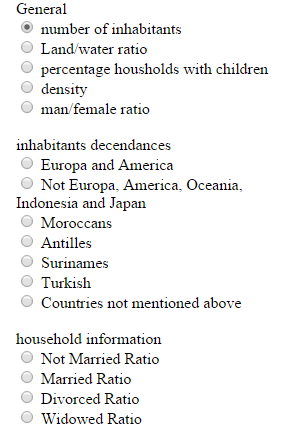
\includegraphics[width=\textwidth]{Interface/HeatmapInterface.png}
                \caption{heatmap interface}
        \end{subfigure}%
        \newline
        \begin{subfigure}[h]{0.34\textwidth}
                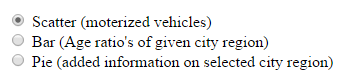
\includegraphics[width=\textwidth]{Interface/VisualizationInterface.png}
                \caption{visualization interface}
        \end{subfigure} \newline
        \caption{Radiobuttons}
\end{wrapfigure}
We decided to use HTML, CSS and JavaScript for the implementation, since the users can visit the visualization easily in their browser, without needing to install additional software. \newline
For the visualization of data, we used the d3.js library. This library allows users to handle data in JavaScript easily. For the visualization we also used the scripts dimple.js and d3pie.js, these use the d3.js library and allow you to take full advantage of the power and flexibility of d3 to visualize data. \newline
We had to use a range of visualizations to display useful data from the given dataset. For this we used the heat map of the Netherlands, a bar chart, a scatter plot and a pie chart. \newline
\begin{wrapfigure}{r}{0.5\textwidth}
        \centering
        \begin{subfigure}[h]{0.12\textwidth}
                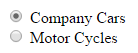
\includegraphics[width=\textwidth]{Interface/ScatterInterface.png}
                \caption{scatter}
        \end{subfigure}
        \begin{subfigure}[h]{0.12\textwidth}
                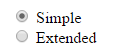
\includegraphics[width=\textwidth]{Interface/BarInterface.png}
                \caption{barchart}
        \end{subfigure}
        \begin{subfigure}[h]{0.12\textwidth}
                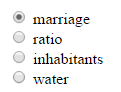
\includegraphics[width=\textwidth]{Interface/PieInterface.png}
                \caption{piechart}
        \end{subfigure}
        \caption{visualization}
\end{wrapfigure}
\subsection{Technical Notes}
We have tested the application in Firefox and Chrome. Other modern browsers like Safari, Opera and Internet Explorer should also support our application, but we have not tested that. \newline
The visualization can be viewed by everyone, if you go to the site "www.isitsunday.com/2IV35.html" (use capital "IV") it will load the visualization we have made for the course 2IV35. How long the link will be supported can not be said at this time. \newline
\subsection{Main Interface}
The interface that is implemented for this visualization is complectly realized with radio buttons. You have the map of the Netherlands with radio buttons on the left side. Using these radio buttons you can make a decision of the data that is represented in the map (a). The map of the Netherlands and the buttons will always be visible, so you are able to change the visualized data on the map. There are also three radio buttons on the top right of the map (b), these allows you to change the visualization that is visible at the left of the map, on default this is the scatter map. However you can change it to bar chart visualization and pie chart visualization. \newline
The radio button interface of the heat map and of the visualization selection can be seen in the figure below and are visible at all times.\newline
There are three visualizations scatter plots, bar charts and pie charts, for every chosen interface a new interface will become visible on the top left of that visualization for these three visualizations the interfaces can be seen in the figure below. \newline
\subsection{HeatMap of the Netherlands}
For this assignment we were provided with some basic code, which used json files to draw the coordinates of the city regions. These regions combined represents the Netherlands. This has been modified in such a way that the city regions change color when hovered over and that every city region is clickable. The map will always be visible in the visualization, because the bar chart and the pie chart require input given from the map. \newline
We have also included multiple datasets to be visualized in the heat map. These have been split in three sections: General, inhabitants descendants and household information sections. \newline
The General section includes: "number of inhabitants"(a), "land/water ratio"(b), "percentage households with children"(c), "density"(d) and "male/female ratio"(e). \newline
The inhabitants descendants section includes: "Europeans and Americans"(f), "Non-Europeans, Americans, Indonesians and Japanese"(g), "Moroccans"(h), "Antillian"(i), "Surinamese"(j), "Turkish"(k) and "Foreigners not mentioned above"(l). \newline
and the household information section includes: "not married ratio"(m), "married ratio"(n), "divorced ratio"(o) and "widowed ratio"(p). The letter after the data represents its location in the figure displaying the heat maps. \newline
We chose this data to be the most interesting and we decided not to add more choices to the list because it would be too much and it would diminish the data that was represented. Data we considered to display but were not included in the age range (a separate heat map for every range). This has already been displayed in the bar chart and the number of cars and motorcycles because it has been visualized in the scatter map. \newline
All the data that has been displayed is shown in the figure below. \newline
\begin{figure}[h]
        \centering
        \begin{subfigure}[b]{0.12\textwidth}
                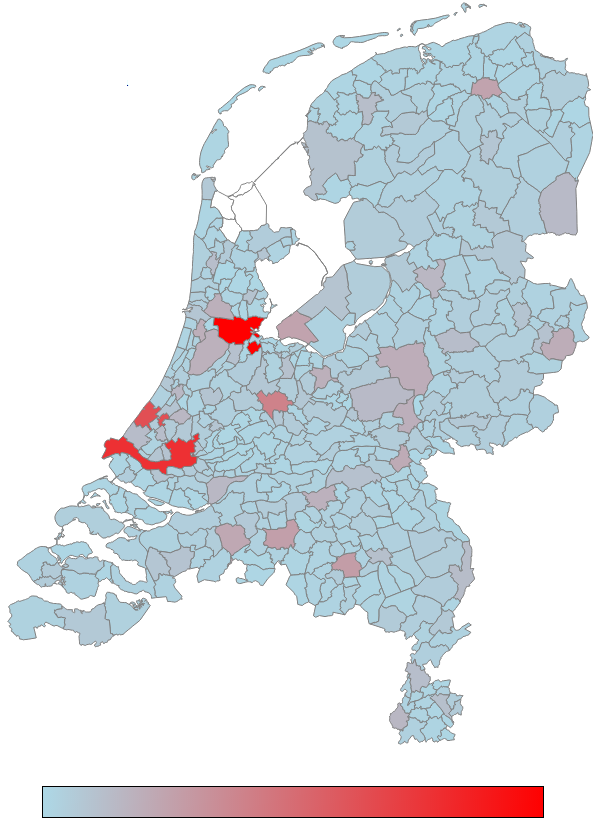
\includegraphics[width=\textwidth]{Heatmaps/HeatMap1.png}
                \caption{}
                \label{fig:numberOfInhabitants}
        \end{subfigure}%
        \begin{subfigure}[b]{0.12\textwidth}
                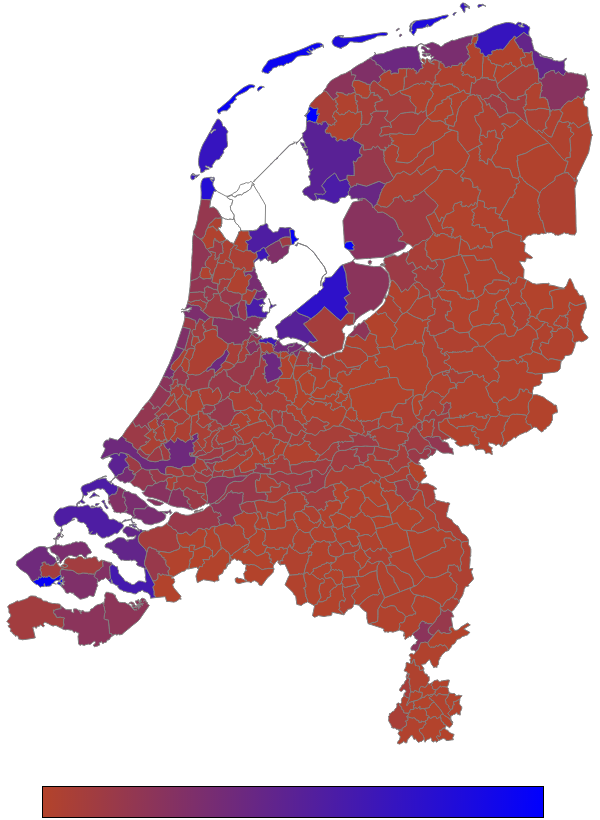
\includegraphics[width=\textwidth]{Heatmaps/HeatMap2.png}
                \caption{}
                \label{fig:LandWater}
        \end{subfigure}
        \begin{subfigure}[b]{0.12\textwidth}
                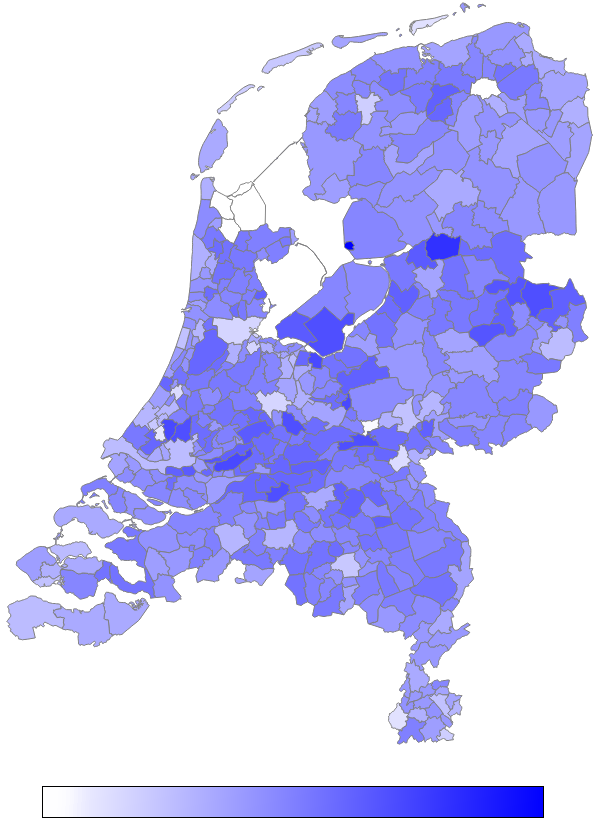
\includegraphics[width=\textwidth]{Heatmaps/HeatMap3.png}
                \caption{}
                \label{fig:HouseholdsChildren}
        \end{subfigure}
        \begin{subfigure}[b]{0.12\textwidth}
                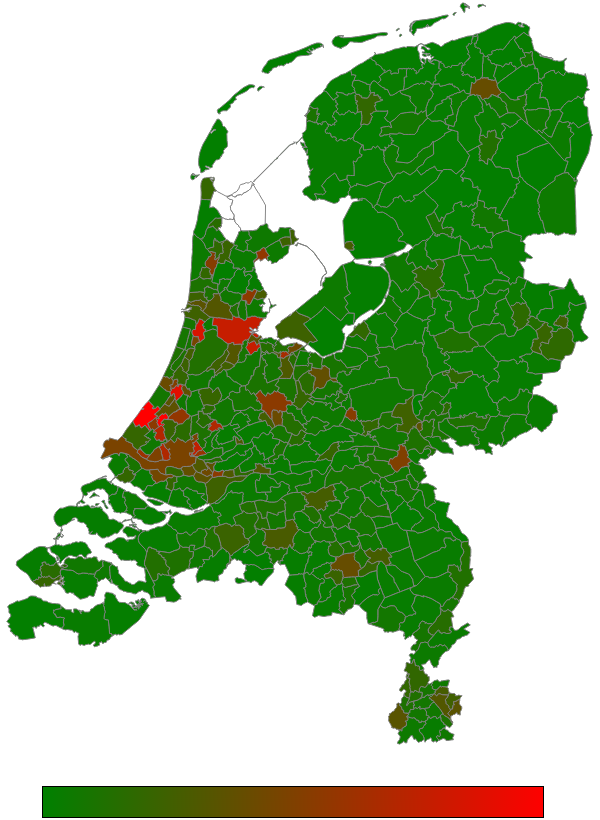
\includegraphics[width=\textwidth]{Heatmaps/HeatMap4.png}
                \caption{}
                \label{fig:Density}
        \end{subfigure}
        \begin{subfigure}[b]{0.12\textwidth}
                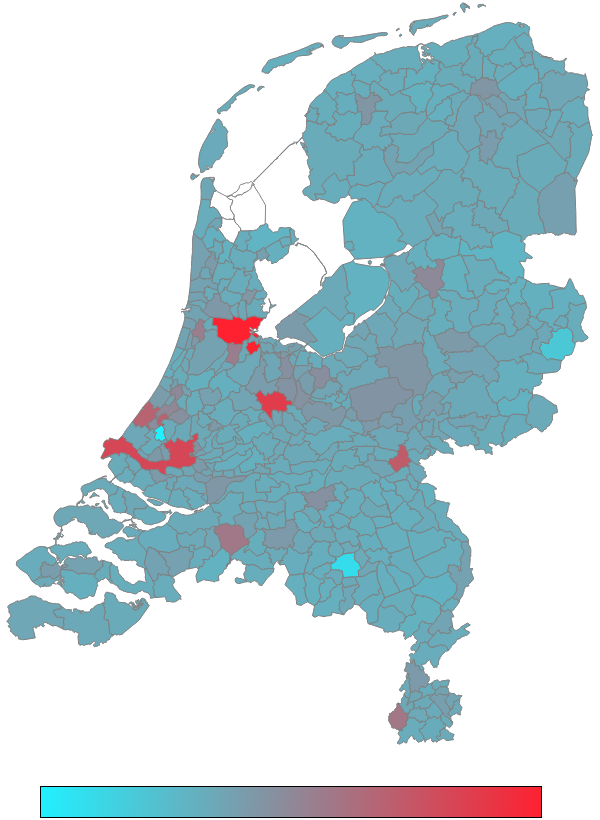
\includegraphics[width=\textwidth]{Heatmaps/HeatMap5.png}
                \caption{}
                \label{fig:MaleFemale}
        \end{subfigure}%
        \begin{subfigure}[b]{0.12\textwidth}
                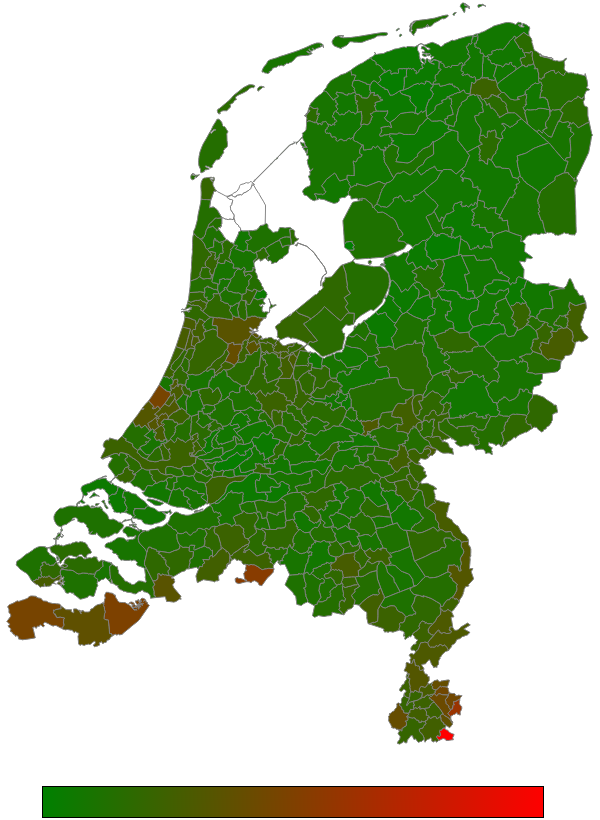
\includegraphics[width=\textwidth]{Heatmaps/HeatMap6.png}
                \caption{}
                \label{fig:EuropeAmerica}
        \end{subfigure}
        \begin{subfigure}[b]{0.12\textwidth}
                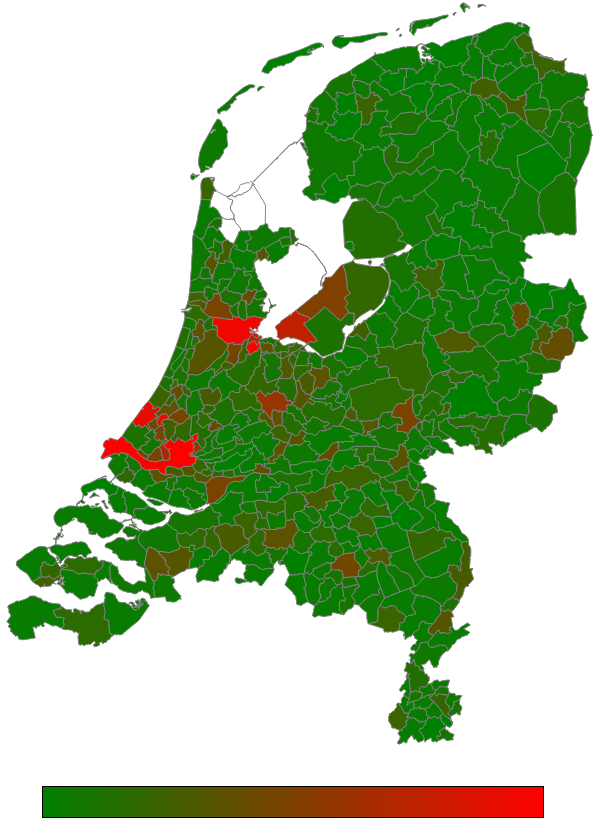
\includegraphics[width=\textwidth]{Heatmaps/HeatMap7.png}
                \caption{}
                \label{fig:notEurope}
        \end{subfigure}
        \begin{subfigure}[b]{0.12\textwidth}
                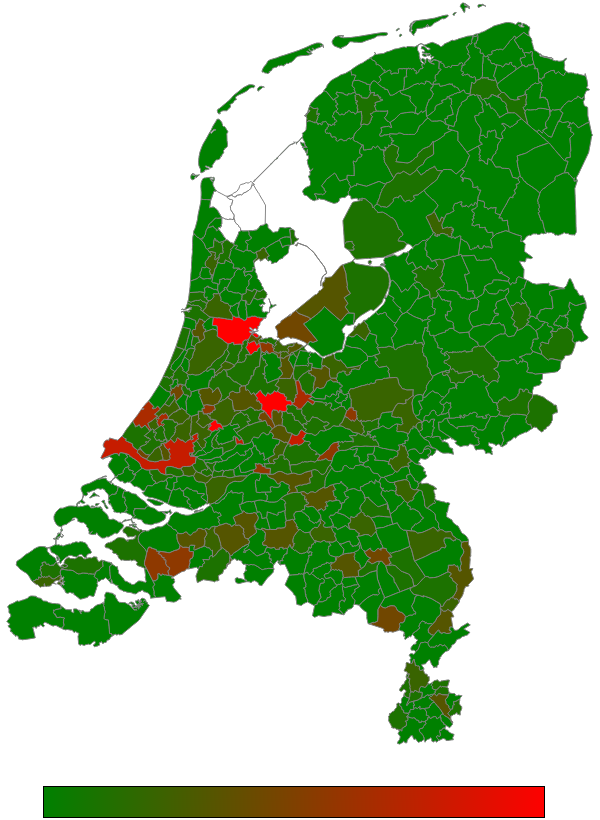
\includegraphics[width=\textwidth]{Heatmaps/HeatMap8.png}
                \caption{}
                \label{fig:Maroccans}
        \end{subfigure} \newline
        \begin{subfigure}[b]{0.118\textwidth}
                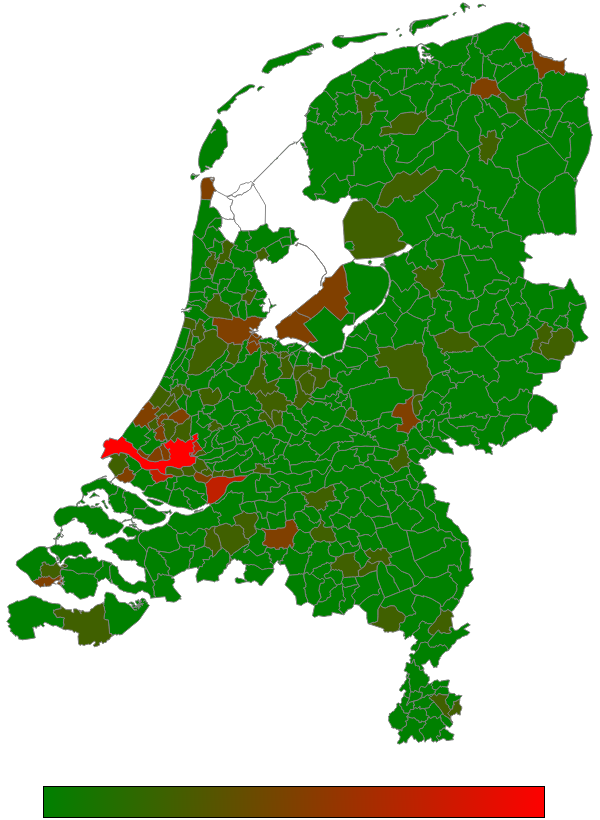
\includegraphics[width=\textwidth]{Heatmaps/HeatMap9.png}
                \caption{}
                \label{fig:Antilles}
        \end{subfigure}%
        \begin{subfigure}[b]{0.118\textwidth}
                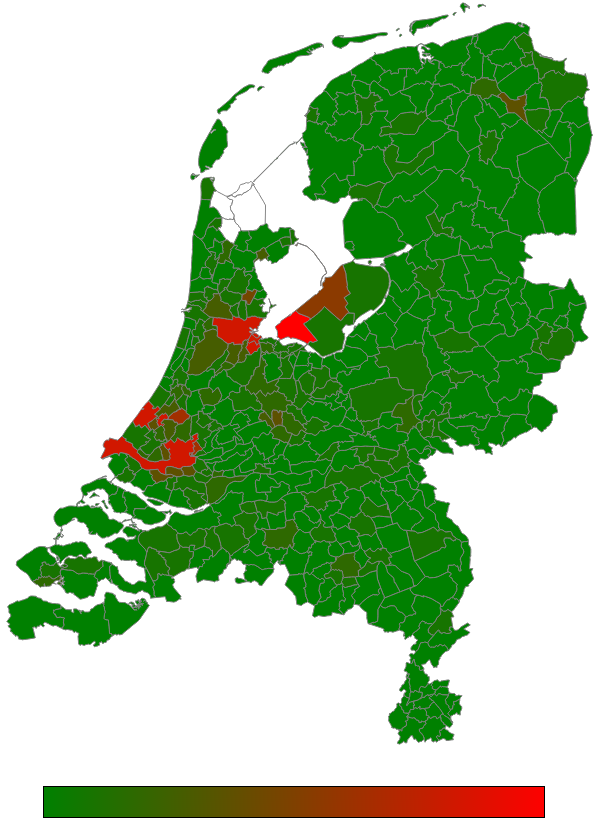
\includegraphics[width=\textwidth]{Heatmaps/HeatMap10.png}
                \caption{}
                \label{fig:Surinames}
        \end{subfigure}
        \begin{subfigure}[b]{0.118\textwidth}
                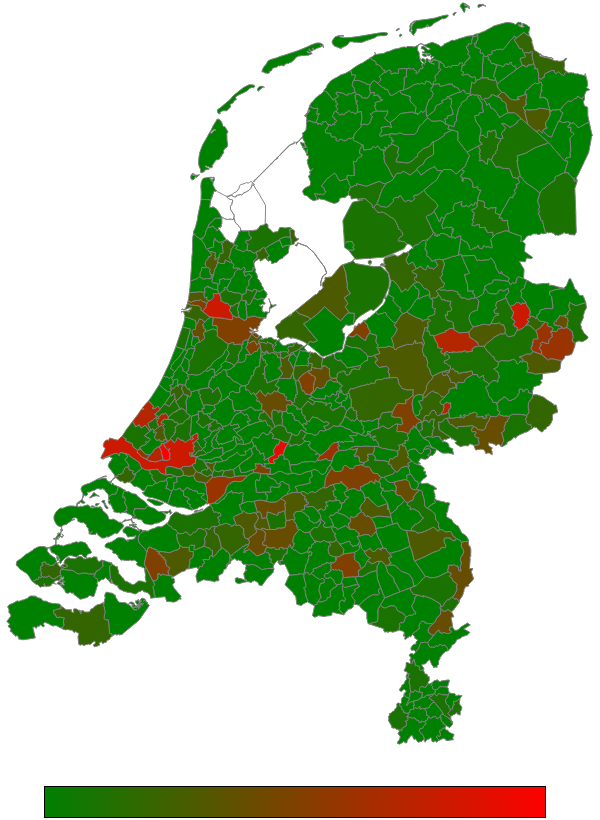
\includegraphics[width=\textwidth]{Heatmaps/HeatMap11.png}
                \caption{}
                \label{fig:Turkish}
        \end{subfigure}
        \begin{subfigure}[b]{0.118\textwidth}
                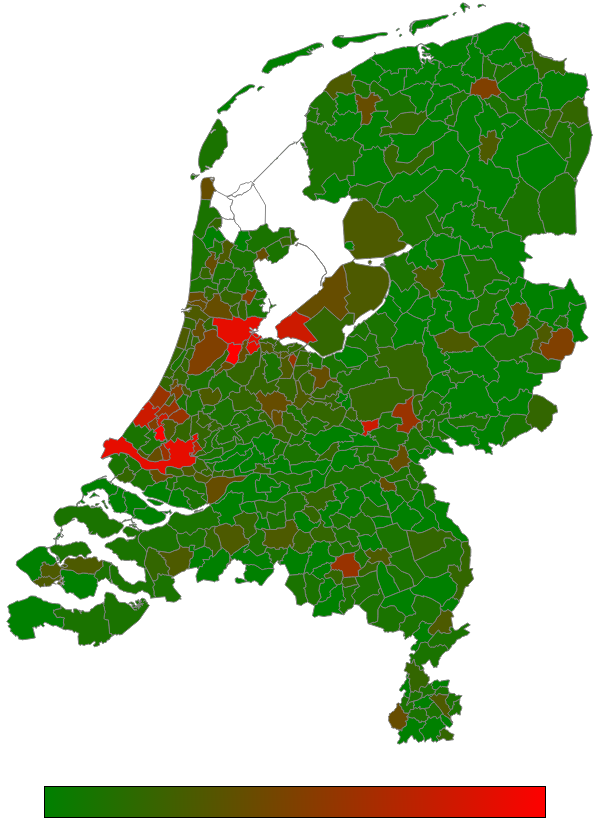
\includegraphics[width=\textwidth]{Heatmaps/HeatMap12.png}
                \caption{}
                \label{fig:notMentioned}
        \end{subfigure}
        \begin{subfigure}[b]{0.118\textwidth}
                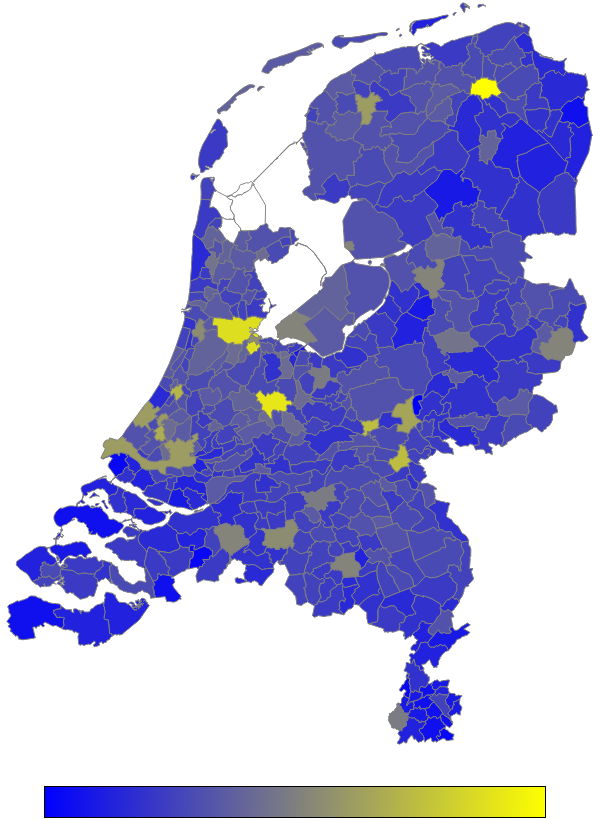
\includegraphics[width=\textwidth]{Heatmaps/HeatMap13.png}
                \caption{}
                \label{fig:notMarried}
        \end{subfigure}
        \begin{subfigure}[b]{0.118\textwidth}
                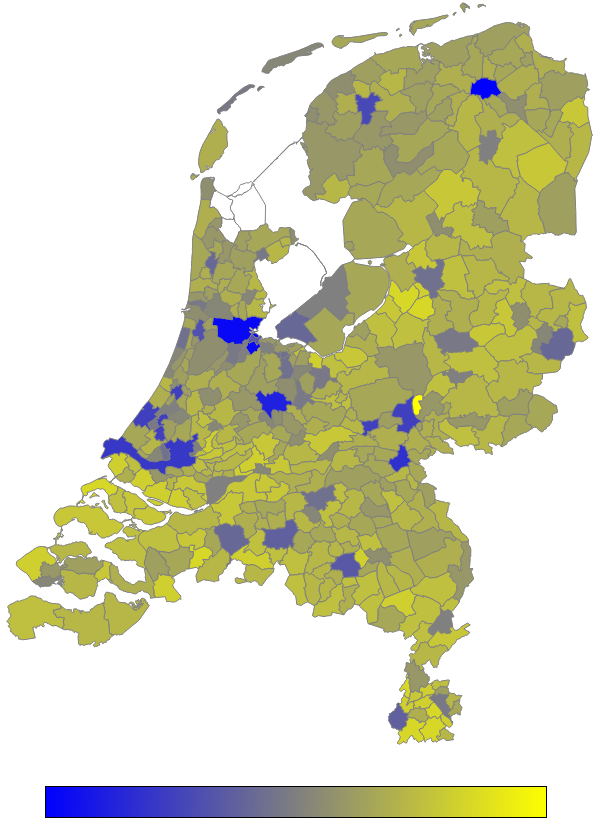
\includegraphics[width=\textwidth]{Heatmaps/HeatMap14.png}
                \caption{}
                \label{fig:Married}
        \end{subfigure}
        \begin{subfigure}[b]{0.118\textwidth}
                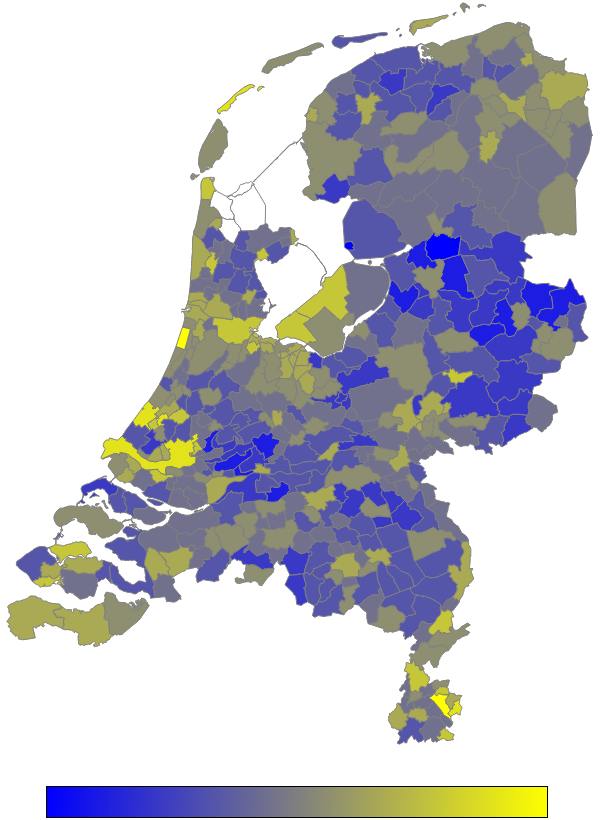
\includegraphics[width=\textwidth]{Heatmaps/HeatMap15.png}
                \caption{}
                \label{fig:Divorced}
        \end{subfigure}
        \begin{subfigure}[b]{0.118\textwidth}
                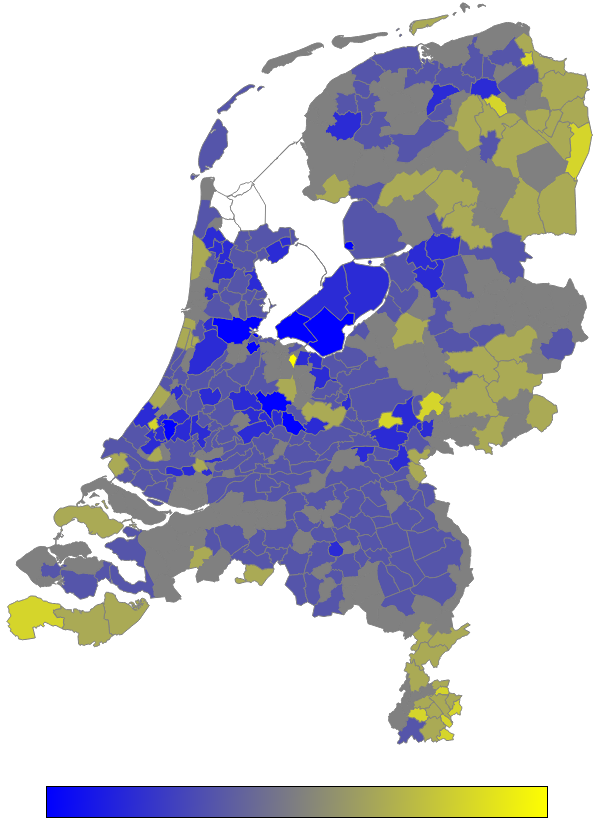
\includegraphics[width=\textwidth]{Heatmaps/HeatMap16.png}
                \caption{}
                \label{fig:Widowed}
        \end{subfigure} \newline
        \caption{All Heatmap visualizations}\label{fig:HeatMaps}
\end{figure}
\subsection{Scatter Plot}
The second visualization which on default is visible when running the site is a scatter plot, there are two options for the scatter plot as explained in the interface chapter, these options are company cars and motorcycles. \newline
When selecting the company cars scatter plot, you will see the scatter plot of the total cars put against the number of company cars, every city region is a bubble and the size of the bubble represents the number of inhabitants. When selecting the Motorcycles the plot is similar, except instead of company cars, the number of motorcycles is displayed. You can hover over a bubble, than a label will appear with the data of that bubble, so the name, inhabitants, total cars and total company cars/motorcycles. A line will be drawn across the x and y axis so you can better determine its location. \newline
The results of the two scatter plots can be seen in the figure below. With the company cars (a) and the motorcycles (b). \newline
\begin{wrapfigure}{r}{1\textwidth}
        \begin{subfigure}[b]{0.5\textwidth}
                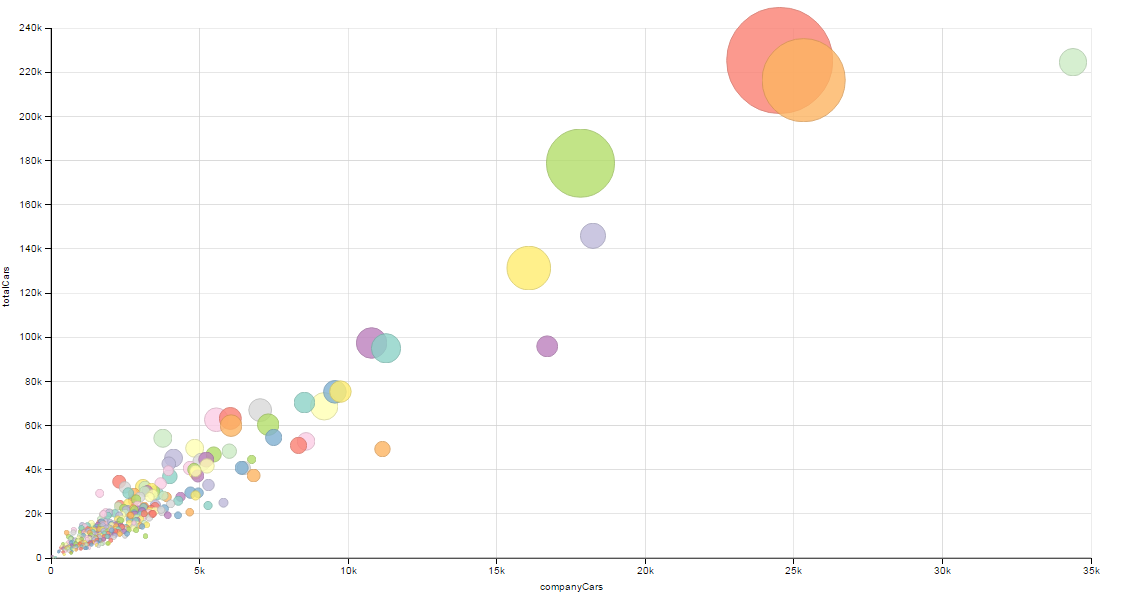
\includegraphics[width=\textwidth]{Visualization/CompanyCars.png}
                \caption{company cars}
                \label{fig:Company}
        \end{subfigure}
        \begin{subfigure}[b]{0.5\textwidth}
                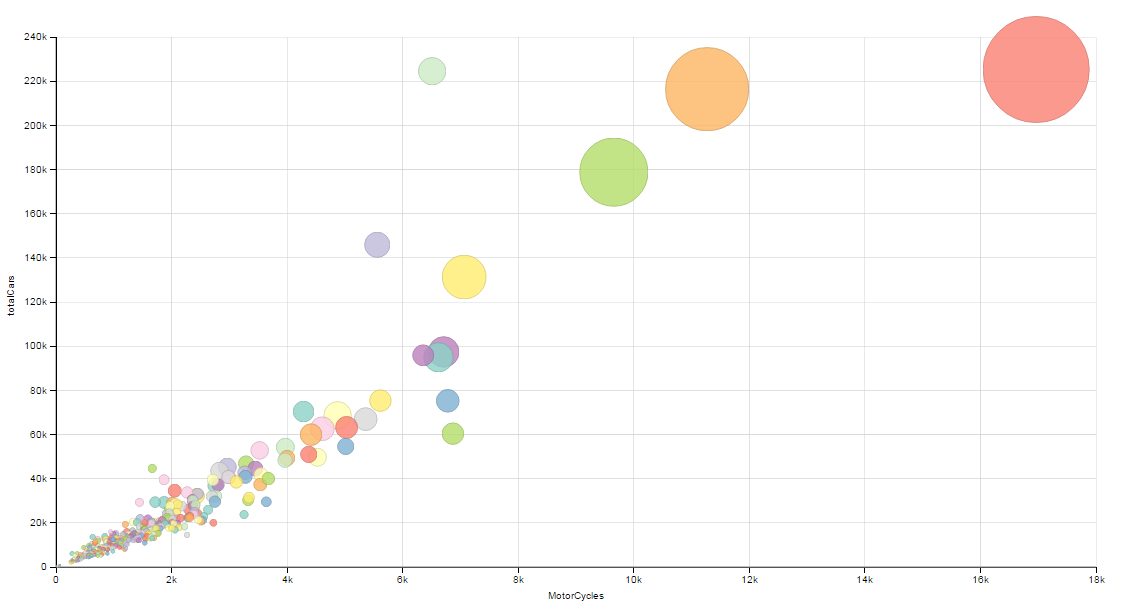
\includegraphics[width=\textwidth]{Visualization/MotorCycles.png}
                \caption{motorcycles}
                \label{fig:MotorCycles}
        \end{subfigure}
        \caption{Scatter plots}\label{fig:scatterPlots}
\end{wrapfigure}
\newline
\newline
\newline
\newline
\newline
\newline
\newline
\newline
\newline
\newline
\newline
\newline
\newline
\subsection{Bar Chart}
The third visualization is a bar chart where the age range percentages are displayed. You can select between simple and extended mode as described in the interface section. The simple chart shows the age range from 0-14 to 65 and older, the extended chart shows the age range from 0 to 4, 5 to 9 all the way to 95 and older. \newline
\newline
\begin{wrapfigure}{r}{1\textwidth}
        \begin{subfigure}[b]{0.23\textwidth}
                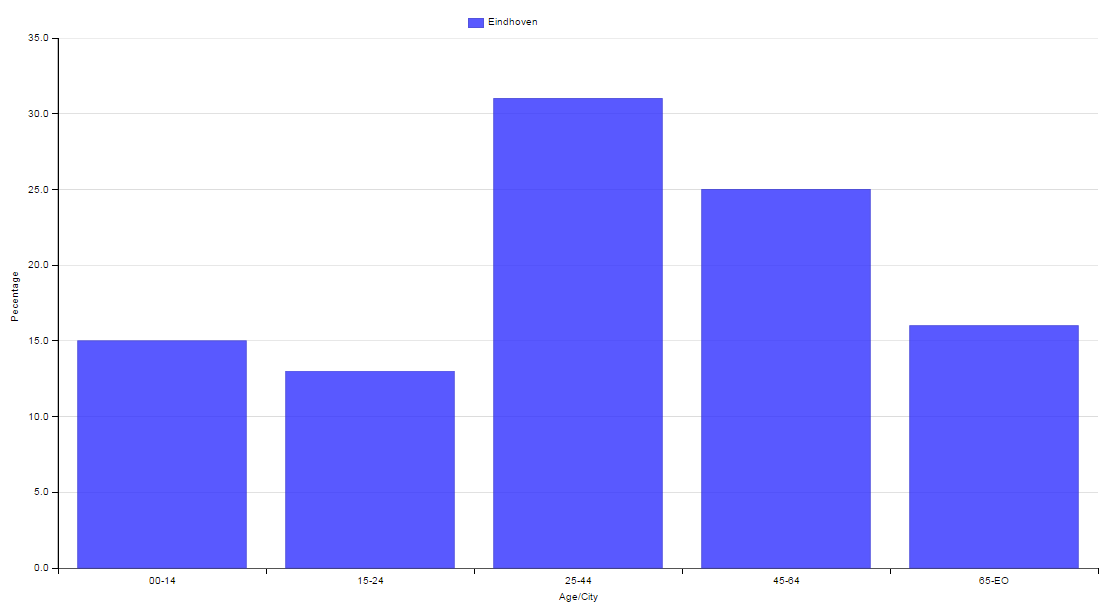
\includegraphics[width=\textwidth]{Visualization/BarChartSimpleSingle.png}
                \caption{small single}
                \label{fig:smallSingle}
        \end{subfigure}
        \begin{subfigure}[b]{0.23\textwidth}
                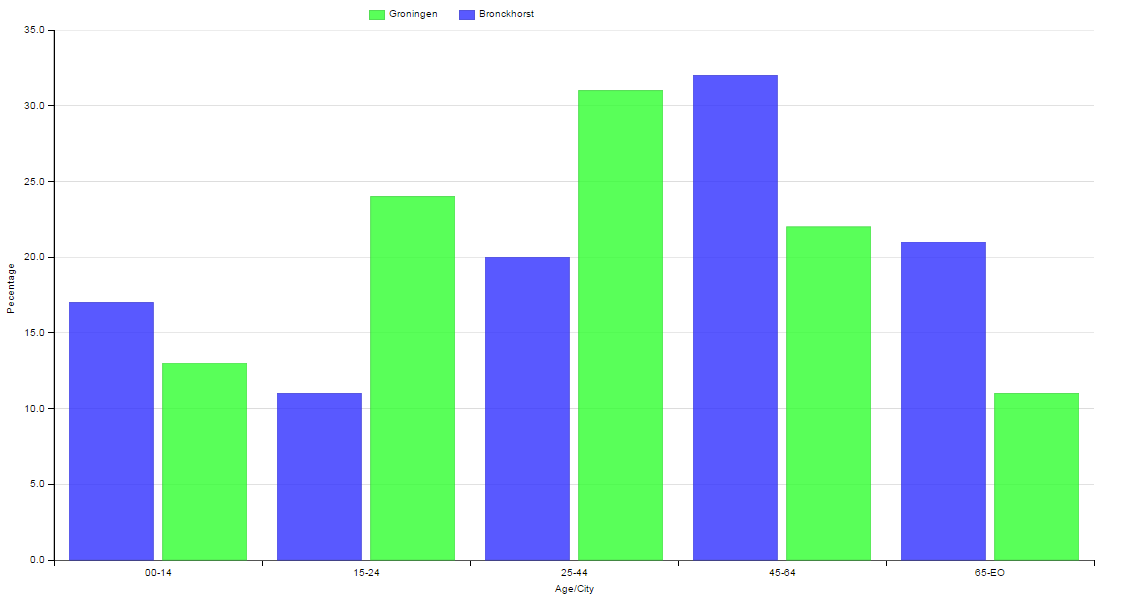
\includegraphics[width=\textwidth]{Visualization/BarChartSimpleFull.png}
                \caption{small extended}
                \label{fig:smallExtended}
        \end{subfigure}
        \begin{subfigure}[b]{0.23\textwidth}
                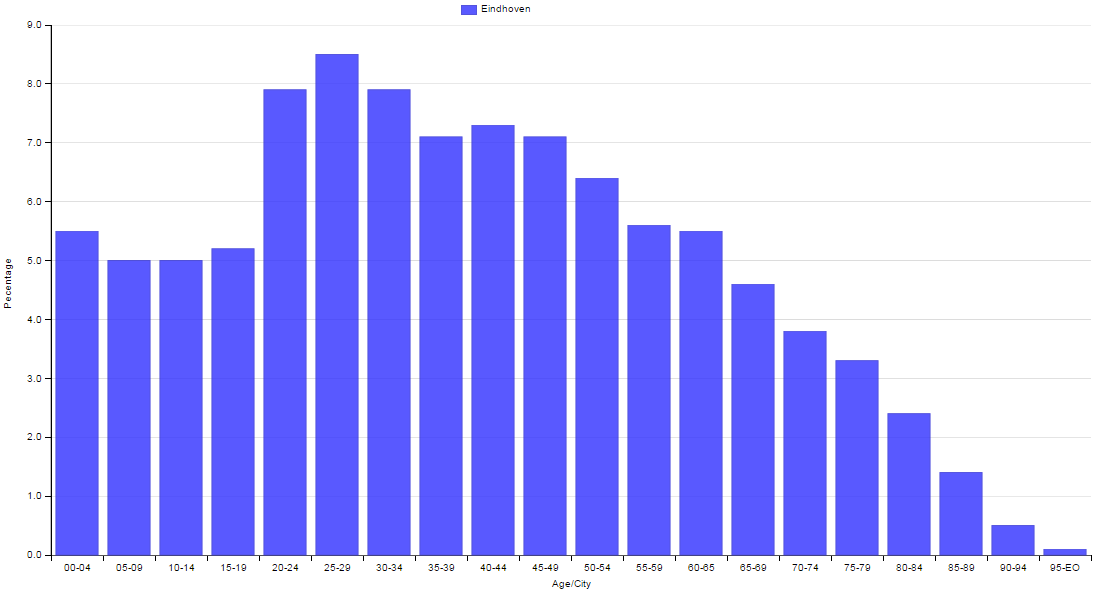
\includegraphics[width=\textwidth]{Visualization/BarChartExtendedSingle.png}
                \caption{big single}
                \label{fig:bigSingle}
        \end{subfigure}
        \begin{subfigure}[b]{0.23\textwidth}
                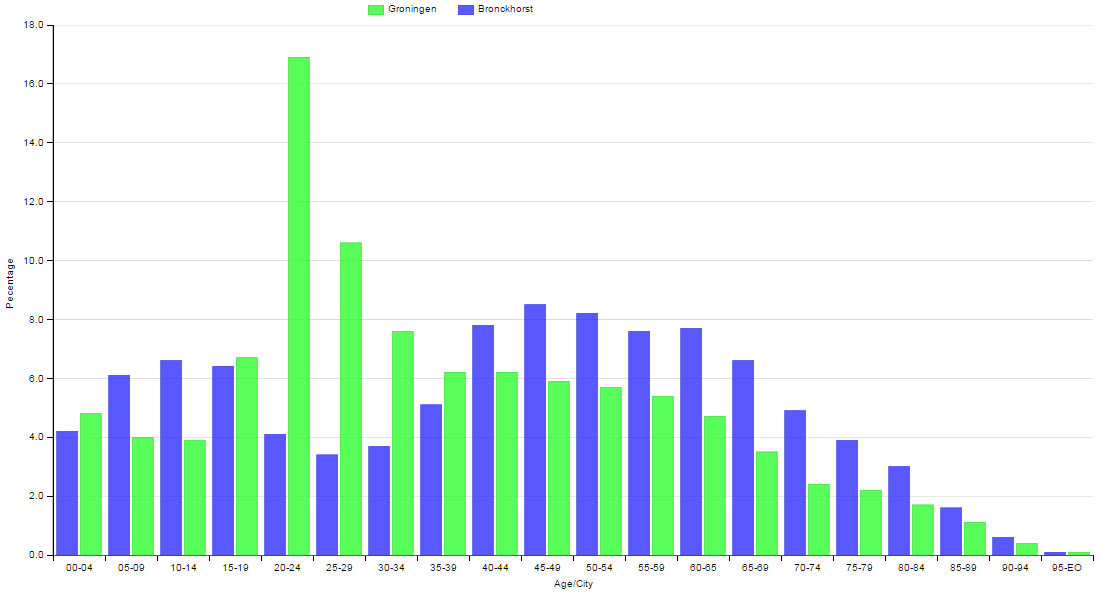
\includegraphics[width=\textwidth]{Visualization/BarChartExtendedFull.png}
                \caption{big extended}
                \label{fig:bigExtended}
        \end{subfigure}
        \caption{Scatter plots}\label{fig:BarCharts}
\end{wrapfigure}
\newline
\newline
\newline
\newline
\newline
\newline
\newline
\newline
\newline
\newline
Selecting a municipality on the map loads the bar chart with the required age data. When a second municipality is selected both the data of the new municipality and the previous one is loaded into the bar chart. Each of these municipalities gets a different color and label to identify them. By double clicking a municipality, you will see only the data of this municipality. \newline
So you can have one city region displayed with simple data (a) or extended data (c), or you can see two city regions next to each other with simple data (b) or with extended data (d) as shown in the figure. \newline
\subsection{Pie Chart}
The fourth visualization is the pie chart where four different kinds of data is visualized, the datasets that are displayed are kept small, because otherwise the pie chart would lose its use. The first data visualized is the marriage data, so the percentage of either married, not married, divorced or widowed inhabitants. The second data that is visualized is the male/female ratio for that city region. The third data is the inhabitants ratio between the last two selected municipalities. And the fourth data is the land/water ratio of the given city regions. \newline
Again you give input by selecting municipalities on the map. The data of the selected municipality is shown in the pie charts. You can switch between the four data options by clicking the radio buttons as described in the interface. In the figure you see an example of the married ratio pie chart (a), the male/female ratio pie chart (b), the inhabitants ratio pie chart (c) and the land/water ratio pie chart.
\begin{wrapfigure}{r}{1\textwidth}
        \begin{subfigure}[b]{0.23\textwidth}
                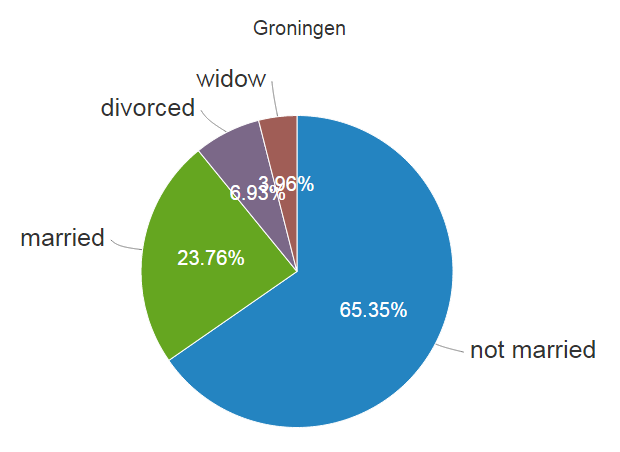
\includegraphics[width=\textwidth]{Visualization/PieChartMarried.png}
                \caption{Married}
                \label{fig:Married}
        \end{subfigure}
        \begin{subfigure}[b]{0.23\textwidth}
                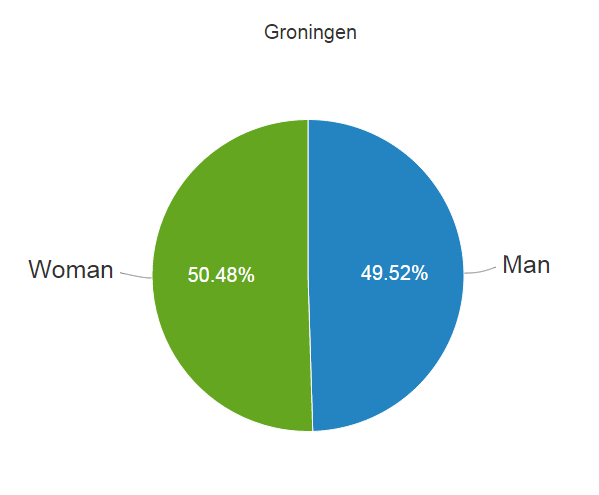
\includegraphics[width=\textwidth]{Visualization/PieChartRatio.png}
                \caption{Male/Female ratio}
                \label{fig:Ratio}
        \end{subfigure}
        \begin{subfigure}[b]{0.2\textwidth}
                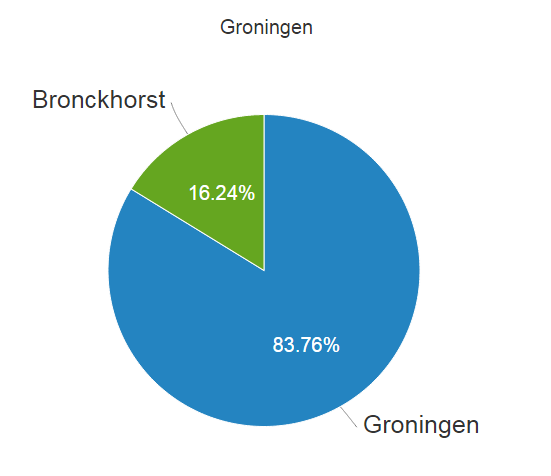
\includegraphics[width=\textwidth]{Visualization/PieChartInhabitants.png}
                \caption{Inhabitants}
                \label{fig:Inhabitants}
        \end{subfigure}
        \begin{subfigure}[b]{0.2\textwidth}
                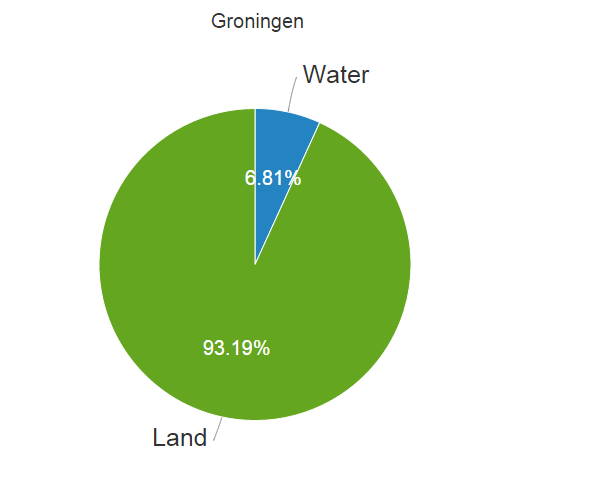
\includegraphics[width=\textwidth]{Visualization/PieChartWater.png}
                \caption{Water ratio}
                \label{fig:Water}
        \end{subfigure}
        \caption{Pie Charts}\label{fig:PieCharts}
\end{wrapfigure}
\newline
\newline
\newline
\newline
\newline
\newline
\newline
\newline
\newline
\newline
\subsection{Hovering and Selecting}
To get more detail from a particular visualization, the user can hover over it with the mouse, this has an effect on visualization. \newline
With the heat map hovering over a city region will color it black, so you know for sure which will be selected when clicking, also if you hold the mouse still over a certain region, you will see the population in that city region and the name of the city region. \newline
With the scatter plot you can mouse over the points in the plot, doing this will drawn lines across the x and y axis so you can easily determine both values. Also a label will appear with all the information about that point, so the name of the city region, inhabitants, total number of cars and the number of company cars/motorcycles. \newline
With the bar chart you can hover over the bars in the plot, the corresponding bar will have a line drawn to the y axis, so you can easily determine the value, also you can see the value in the label which will be shown when hovering over it, this gives the percentage of that bar and the given value of the x axis, with the name of the city region. \newline
With the pie chart you can click on a pie section of the chart, this will cause the slice to pop out so you can better determine the size, also the actual percentage is displayed in the slice. \newline
\newpage

\section{Trends}
We have used our application to analyze the data and found a couple of trends. By
this we mean remarkable changes or values in the data. \newline \newline
The first trend we found was that there is a direct correlation between the number of inhabitants and cars within a municipality. However there is a obvious outlier and that is Almere, since it has lots of motorcycles in contrast to the number of inhabitants. For a reason we think that there are many lease companies located there. \newline \newline
The second trend is that the most widowers are located near the borders of the Netherlands. We could not find a good reason for that. However if you compare the number of widowers to the age in the municipality you can easily find that the average age of these municipality is higher to the one without many widowers. \newline \newline
A third trend is that most foreigners live in the larger cities like Rotterdam, Amsterdam and Utrecht.
\newpage
\section{Conclusion}
In this chapter we review the results of our visualizations. \newline
The scatter plot is a good decision since it shows a lot of data in one view. However, since most cities clutter in the left corner a part of the information is lost. We could improve this by making a selection of points possible and add zooming. \newline
The bar chart displays the age categories very clearly. But also here we could improve by for example adding a average age line to it. An other improvement could be that instead of just clicking simple and extended view to unfold just a selected age bar in subcategories. This way you enable the users to directly search for the data. \newline
Overall we think our visualizations suits the data good. We can easily find the answers of different questions. Nevertheless we think that the interface could be improved more. In some cases it is not directly clear what municipality is selected, since this is not reflected in the map. Also a clear flow of the application is missing. With this we mean that each view shows different information, we could improve by showing the same information in different views. An approach like this gives the users the power to select the best view for the data, instead of that the developer makes these discission for them. Naturally this dependents on the target group of your application.

\subsection{Testing}
We tested our application with a select group of people and asked them to find the municipality with the most woman between the age of 20 to 25. They came up with Utrecht and Nijmegen as the correct municipalities. So they successfully answered the question in little time. The test group was very interested in our visualization and liked to discover the data in the manner it was presented them.

\begin{figure}[h]
        \centering
        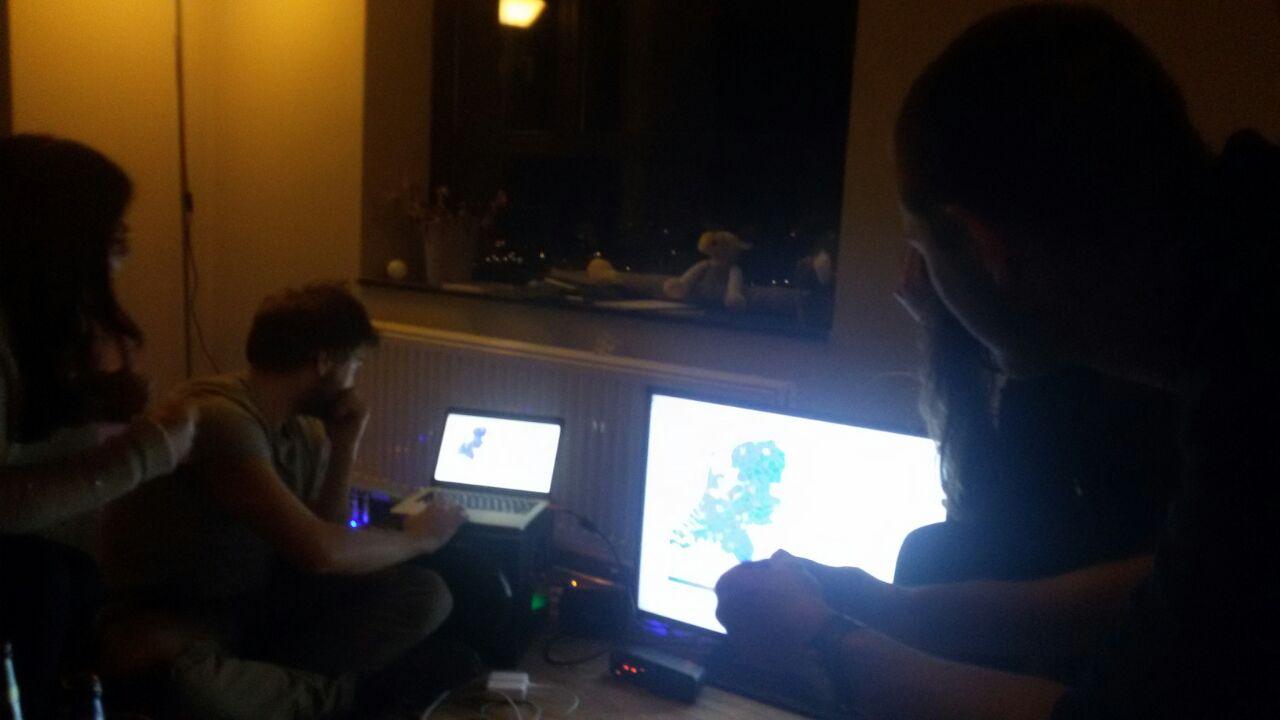
\includegraphics[width=\textwidth]{Conclusion/Conclusion1.jpg}
        \caption{Visualization testing group}
        \label{fig:numberOfInhabitants}
\end{figure}



\end{document} 